
\lecture{Lecture - 26\hfill 28 Oct 24, Mon}

\begin{definition}[Tree]
	A tree is a connected grpah with no cycles.
\end{definition}
\begin{definition}[Forest]
	A forst is a graph with no cycles, or an acyclic graph.
\end{definition}
The connected components of a forest are trees.
\begin{example}
	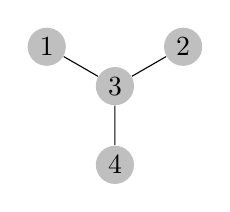
\begin{tikzpicture}
		\tikzstyle{vertex}=[circle,fill=black!25,minimum size=12pt,inner sep=2pt]
		\node[vertex] (g_1) at (150:1) {1};
		\node[vertex] (g_2) at (30:1) {2};
		\node[vertex] (g_3) at (0,0) {3};
		\node[vertex] (g_4) at (270:1) {4};
		\draw (g_3) -- (g_1) (g_3) -- (g_2) (g_3) -- (g_4);
	\end{tikzpicture}
is a tree.

	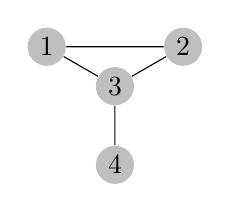
\begin{tikzpicture}
		\tikzstyle{vertex}=[circle,fill=black!25,minimum size=12pt,inner sep=2pt]
		\node[vertex] (g_1) at (150:1) {1};
		\node[vertex] (g_2) at (30:1) {2};
		\node[vertex] (g_3) at (0,0) {3};
		\node[vertex] (g_4) at (270:1) {4};
		\draw (g_3) -> (g_1) (g_1) -> (g_2) (g_2) -> (g_3) (g_3) -- (g_4);
	\end{tikzpicture}
	is not a tree.
\end{example}

\begin{definition}[Leaf]
	For a graph $G,$ a leaf is a vertex of degree 1.
\end{definition}
Given a graph $G = (V, E),$ and a subset $A$ of $V,$ the induced 
subgraph on $V \setminus A$ 
$$ \left( V \setminus A, E \setminus \{e \in E \; : \; 
\text{ both ends of } e \text{ are in } V\setminus A \} \right).$$
\begin{lemma}
	Let $T$ be a tree with $n \geq 2$ vertices. Then
\begin{enumerate}
	\item $T$ contains at least $2$ leaves.
	\item For any leaf $i$ in $G,$ $T \setminus \{i\}$ is a tree
		with $n-1$ vertices.
\end{enumerate}
\end{lemma}
\begin{proof}
	Let $P$ be a maximal path in $T,$ that is, adding any edges
	to $P$ results in a walk which is not a path. Let $v_0,$ 
	$v_k$ be the starting point and ending point of $P.$ Then
	every neighbour of $v_0$ and $v_k$ must be in $P,$ by
	maximality of $P.$ As $v_0$ is the starting point, at most
	one of its neighbours is in $P.$ This is because every vertex
	$v$ in $P$ appears in $P$ exactly once. So, $v_0$ has exactly
	one neighbour. Similarly, $v_k$ also has exactly one neighbour.
	Indeed, $v_0$ and $v_k$ have to have at least one neighbour
	because $T$ is a tree. This shows that $v_0$ and $v_k$ are
	leaves.

Let $i$ be a leaf in $T.$ Then $T \setminus \{i\}$ is acyclic because
$T$ is acyclic. Let $l$ and $k$ be vertices in $T \setminus \{i\}.$
There exists a path $P$ in $T$ from $l$ to $k.$ Then $P$ does not
contain $i$ because if a vertex $v$ is not an endpoint of $P,$ then
it must have two distinct neighbours and $i$ is not an endpoint.
\end{proof}

\begin{theorem}[Characterisation of Trees]
	Let $T = (V, E)$ be a graph on a $n$ vertices. Then the 
	following statements are equivalent. 
\begin{enumerate}
	\item $T$ is a tree.
	\item $T$ is connected and has $n-1$ edges.
	\item $T$ has $n-1$ edges and no cycles.
	\item For any distinct vertices $i, j$ in $V,$ there exists
		a unique path from $i$ to $j.$
\end{enumerate}
\end{theorem}
In other words, any two of the three properties acyclicity, 
connectedness, and $\lvert V \rvert - \lvert E \rvert = 1,$
imply the third.
\begin{proof}
	We will try to show that $(1) \implies (2) \implies (3) \implies
	(1)$ and $(1) \iff (4).$ 
	$(1) \implies (2)$ can be shown using induction. For $n=1$ and 
	$2,$ the lemma holds because the only trees with $1,$ or $2$
	vertices are
\begin{figure}[h]
\centering
\begin{tikzpicture}
	\node (v1) at (0,0) {1};
	\node (v2) at (1,0) {2};
	\draw (v1) -- (v2);
\end{tikzpicture}
\end{figure}
and the trivial tree with $1$ vertex.
As we have shown previously that $T$ must have at least one leaf, 
we can assume that there exists a leaf $i$ in $G.$ Then $T \setminus
\{i\}$ is also a tree and has $n-2$ edges, by induction hypothesis.
This shows that $T$ has $n-1$ edges.

To show that $(2) \implies (3),$ we assume that $T$ has $n-1$ edges
and is cyclic. Then, removing some edges from $T$ results in an
induced subgraph $T'$ which is acyclic but no connected component
becomes disconnected. As $T'$ has fewer than $n-1$
edges, it can not be connected, for a tree with $n$ vertices
necessarily has $n-1$ edges. This means that $T$ is not connected
because $T$ and $T'$ have equally many components.

\end{proof}
